\documentclass[a4paper,10pt]{article}

\usepackage{fullpage}
\usepackage[spanish]{babel}
\usepackage{cite}
\usepackage[utf8]{inputenc}
\usepackage{a4wide}
\usepackage{url}
\usepackage{graphicx}
\usepackage{caption}
\usepackage{float} % para que los gr\'aficos se queden en su lugar con [H]
\usepackage{subcaption}
\usepackage{wrapfig}
\usepackage{color}
\usepackage{amsmath} %para escribir funci\'on partida , matrices
\usepackage{amsthm} %para numerar definciones y teoremas
\usepackage{hyperref} % para inlcuir links dentro del texto
\usepackage{tabu} 
\usepackage{comment}
\usepackage{amsfonts} % mathbb{N} -> conjunto de los n\'umeros naturales  
\usepackage{enumerate}
\usepackage{listings}
\usepackage{todonotes} % Para poner notas en el medio del texto!! No olvidar hacer. 
\usepackage{framed} % Para encuadrar texto. \begin{framed}
\usepackage{csquotes} % Para citar texto \begin{displayquote}
\usepackage{epigraph} % Epigrafe  \epigraph{texto}{\textit{autor}}

\usepackage{titlesec}


\newtheorem{midef}{Definition}
\newtheorem{miteo}{Theorem}

\definecolor{dkgreen}{rgb}{0,0.6,0}
\definecolor{gray}{rgb}{0.5,0.5,0.5}
\definecolor{mauve}{rgb}{0.58,0,0.82}

\lstset{frame=tb,
  language=Sql,
  aboveskip=3mm,
  belowskip=3mm,
  showstringspaces=false,
  columns=flexible,
  basicstyle={\small\ttfamily},
  numbers=none,
  numberstyle=\tiny\color{gray},
  keywordstyle=\color{blue},
  commentstyle=\color{dkgreen},
  stringstyle=\color{mauve},
  breaklines=true,
  breakatwhitespace=true,
  tabsize=2
}

\title{Aprendizaje autom\'atico}
\author{Grupo Sociof\'isica \\
Sebasti\'an Pinto, Guillermo Pasqualetti, Gustavo Landfried}

\begin{document}

\maketitle

\section{Introducci\'on}

Usamos el lenguaje de progrmaci\'on python. 

Usamos conceptos del libro ``An Introduction to Statistical Learning''~\cite{james_hastie_tibshirani}.

\section{Extracci\'on de atributos}

\par Identificamos 127 atributos para la clasificación del mail, los cuales constituyeron dos grupos: características del texto y palabras involucradas. Dentro de las características del texto elegimos:
\begin{itemize}
\item La diferencia sim\'etrica de los conjuntos de palabras m\'as frecuentes en \emph{spam} y \emph{ham}
\item Palabras reportadas en dos papers \cite{Gunal} y \cite{Vaughan}. 
\item Largo del documento.
\item Cantidad de espacios en blanco.
\item Si el archivo contiene o no html.
\item Si el mail es una respuesta.
\item Cantidad de caracters no ASCII.
\end{itemize}
La hipótesis detrás de dichas elecciones es que un mail clasificado como \emph{spam} es más probable que contenga un archivo \emph{html} y una mayor cantidad de caracteres no ASCII, como sucede en el empleo de idiomas que no sea el inglés. Por otro lado, en un mail etiquetado como \emph{ham} esperamos que tenga un largo menor que \emph{spam}, que haya grandes diferencias en el empleo de uso de espacios en blanco, y si el mail es una respuesta, probablemente provenga de una conversación entre dos usuarios reales.
\par La elección de palabras involucradas se basó a su vez en dos criterios separados: por un lado incluimos un listado de palabras propuestas por los trabajos \cite{Gunal} y \cite{Vaughan}, que fueron catalogadas como buenas discriminadoras entre mails \emph{ham} y \emph{spam}, y por otro lado, mediante la librería de python \emph{nltk} (\cite{nltk}), extraímos los 25 términos más frecuentes del dataset tanto para \emph{ham} como para \emph{spam}. El atributo entonces elegido es la cantidad de veces que aparece una dada palabra en el texto.


\section{Modelos}

\subsection{Decision Tree Classifier. DTC.}

\par Con la finalidad de escoger el mejor árbol de desición exploramos 
el desempeño sobre los datos de entrenamiento en una grilla de híper-parámetros.
De entre el total de híper-parametros del modelo decidimos profundizar sobre 
tres que nos parecieron especialmente relevantes:
\begin{itemize}
 \item Profundidad máxima [Valor entero]: Máxima profundidad del árbol de desición. 
 \item Criterio Gini Impurity  Information Gain: función que mide la cualidad 
del ``split''. 
  \item Splitter Best  Random: estrategia usada para elegir el mejor 
``split'' en cada nodo.
\end{itemize}

Los híper-parametros ``Criterio'' y ``Splitter'' no tuvieron un impacto 
significativo en la performance; para ellos escogimos los valores Gini Impurity 
y Best, respectivamente.
El híper parametro ``Profundidad máxima'' tuvo, en cambio, un impacto 
importante sobre el desempeño. La figura siguiente muestra 
la relación funcional entre ambos.

  \begin{figure}[H]
    \centering
    \begin{subfigure}[b]{0.4\textwidth}
      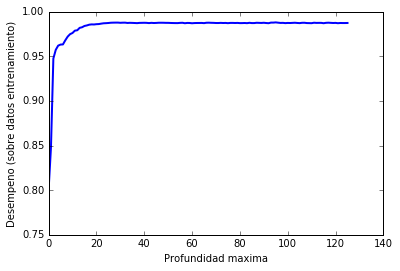
\includegraphics[width=\textwidth]{../imagenes/desempeno-profundiad_arboles}
      \caption{}
    \end{subfigure}
    \label{fig:autovalores}
  \end{figure}


Vemos que el desempeño presenta una fuerte mejora con la profundidad máxima 
permitida al árbol hasta profundidades de 15 a 20 niveles. Luego el desempeño 
prácticamente no crece. Para evitarnos posibles problemas de 'overfitting', 
decidimos limitar en 15 la profundidad de los árboles usados con un desempeño 
correspondiente de 0.982.

\subsection{Naive Bayes. NB.}

El m\'etodo Naive Bayes no result\'o adecuado para este set de datos. El desempeño 
sobre los datos de entrenamiento fue de tan solo 0.524. 


\todo[inline]{¿Por qu\'e creemos el desepeño de NB fue tan malo?. Gustavo: a mi se me ocurre que las variables son demasiado dependientes entre s\'i, lo cual \'indicar\'ia un problema con las variables que tomamos}


\subsection{k-nearest neighbors. KNN}

Probamos el m \'etodo de los vecinos m\'as cercanos. Para determinar la cantidad de vecinos \'optimo hicimos cross validation con 10-folds con 1,10,20,40,80,160,320,640 vecinos. Los resultados son los siguientes, 

\begin{figure}[H]
  \centering
  \begin{subfigure}[b]{0.4\textwidth}
    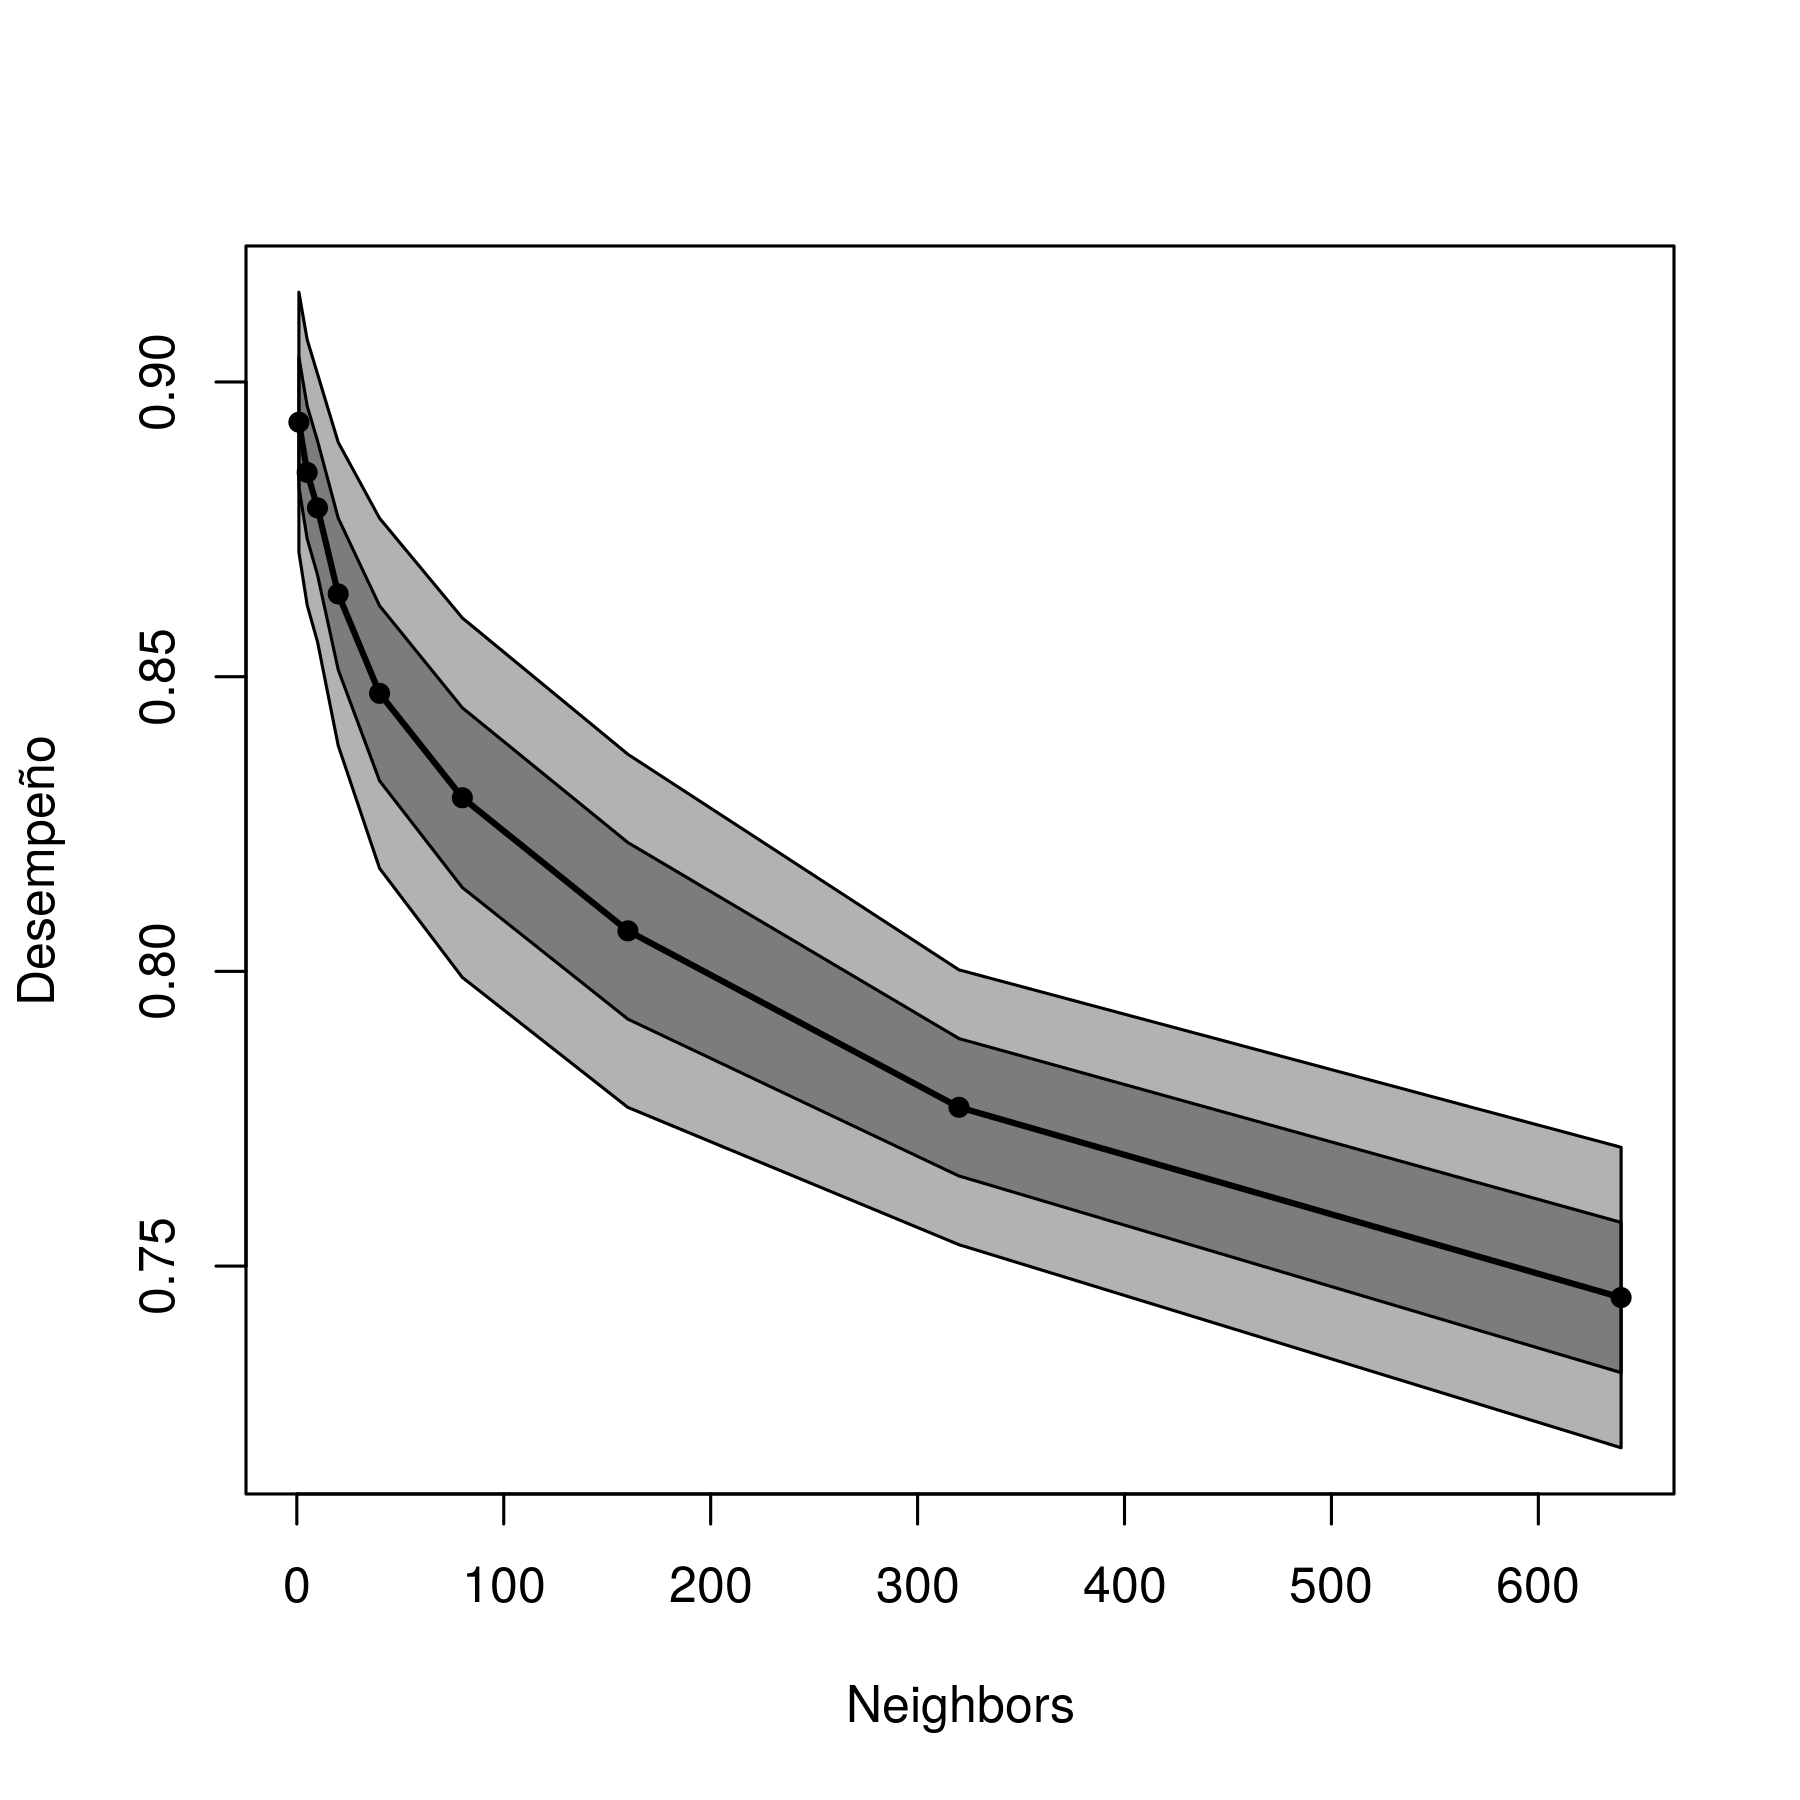
\includegraphics[width=\textwidth]{../imagenes/knn-n_neighbors}
     \caption{}
  \end{subfigure}
  \label{fig:knn-n_neighbors}
\end{figure}

El desempeño m\'aximo, menor a 0.9, result\'o ser bajo en comporaci\'on con otro m\'etodos. Nos sorprendi\'o particularmente que la cantidad de vecinos \'optimo para este problema haya sido con un \'unico vecino. 

\todo[inline]{¿Por qu\'e creemos que k=1 result\'o ser la cantidad \'optima de vecinos?. Gustavo: a mi se me ocurre que las variables no agrupan las instancias en espacios bien definidos, sino que se intercalan. Esto indicar\'ia que un problema con las variables que tomamos.}



\subsection{Random Forest. RF.}

Los \'arboles generados. 

\begin{figure}[H]
  \centering
  \begin{subfigure}[b]{0.4\textwidth}
    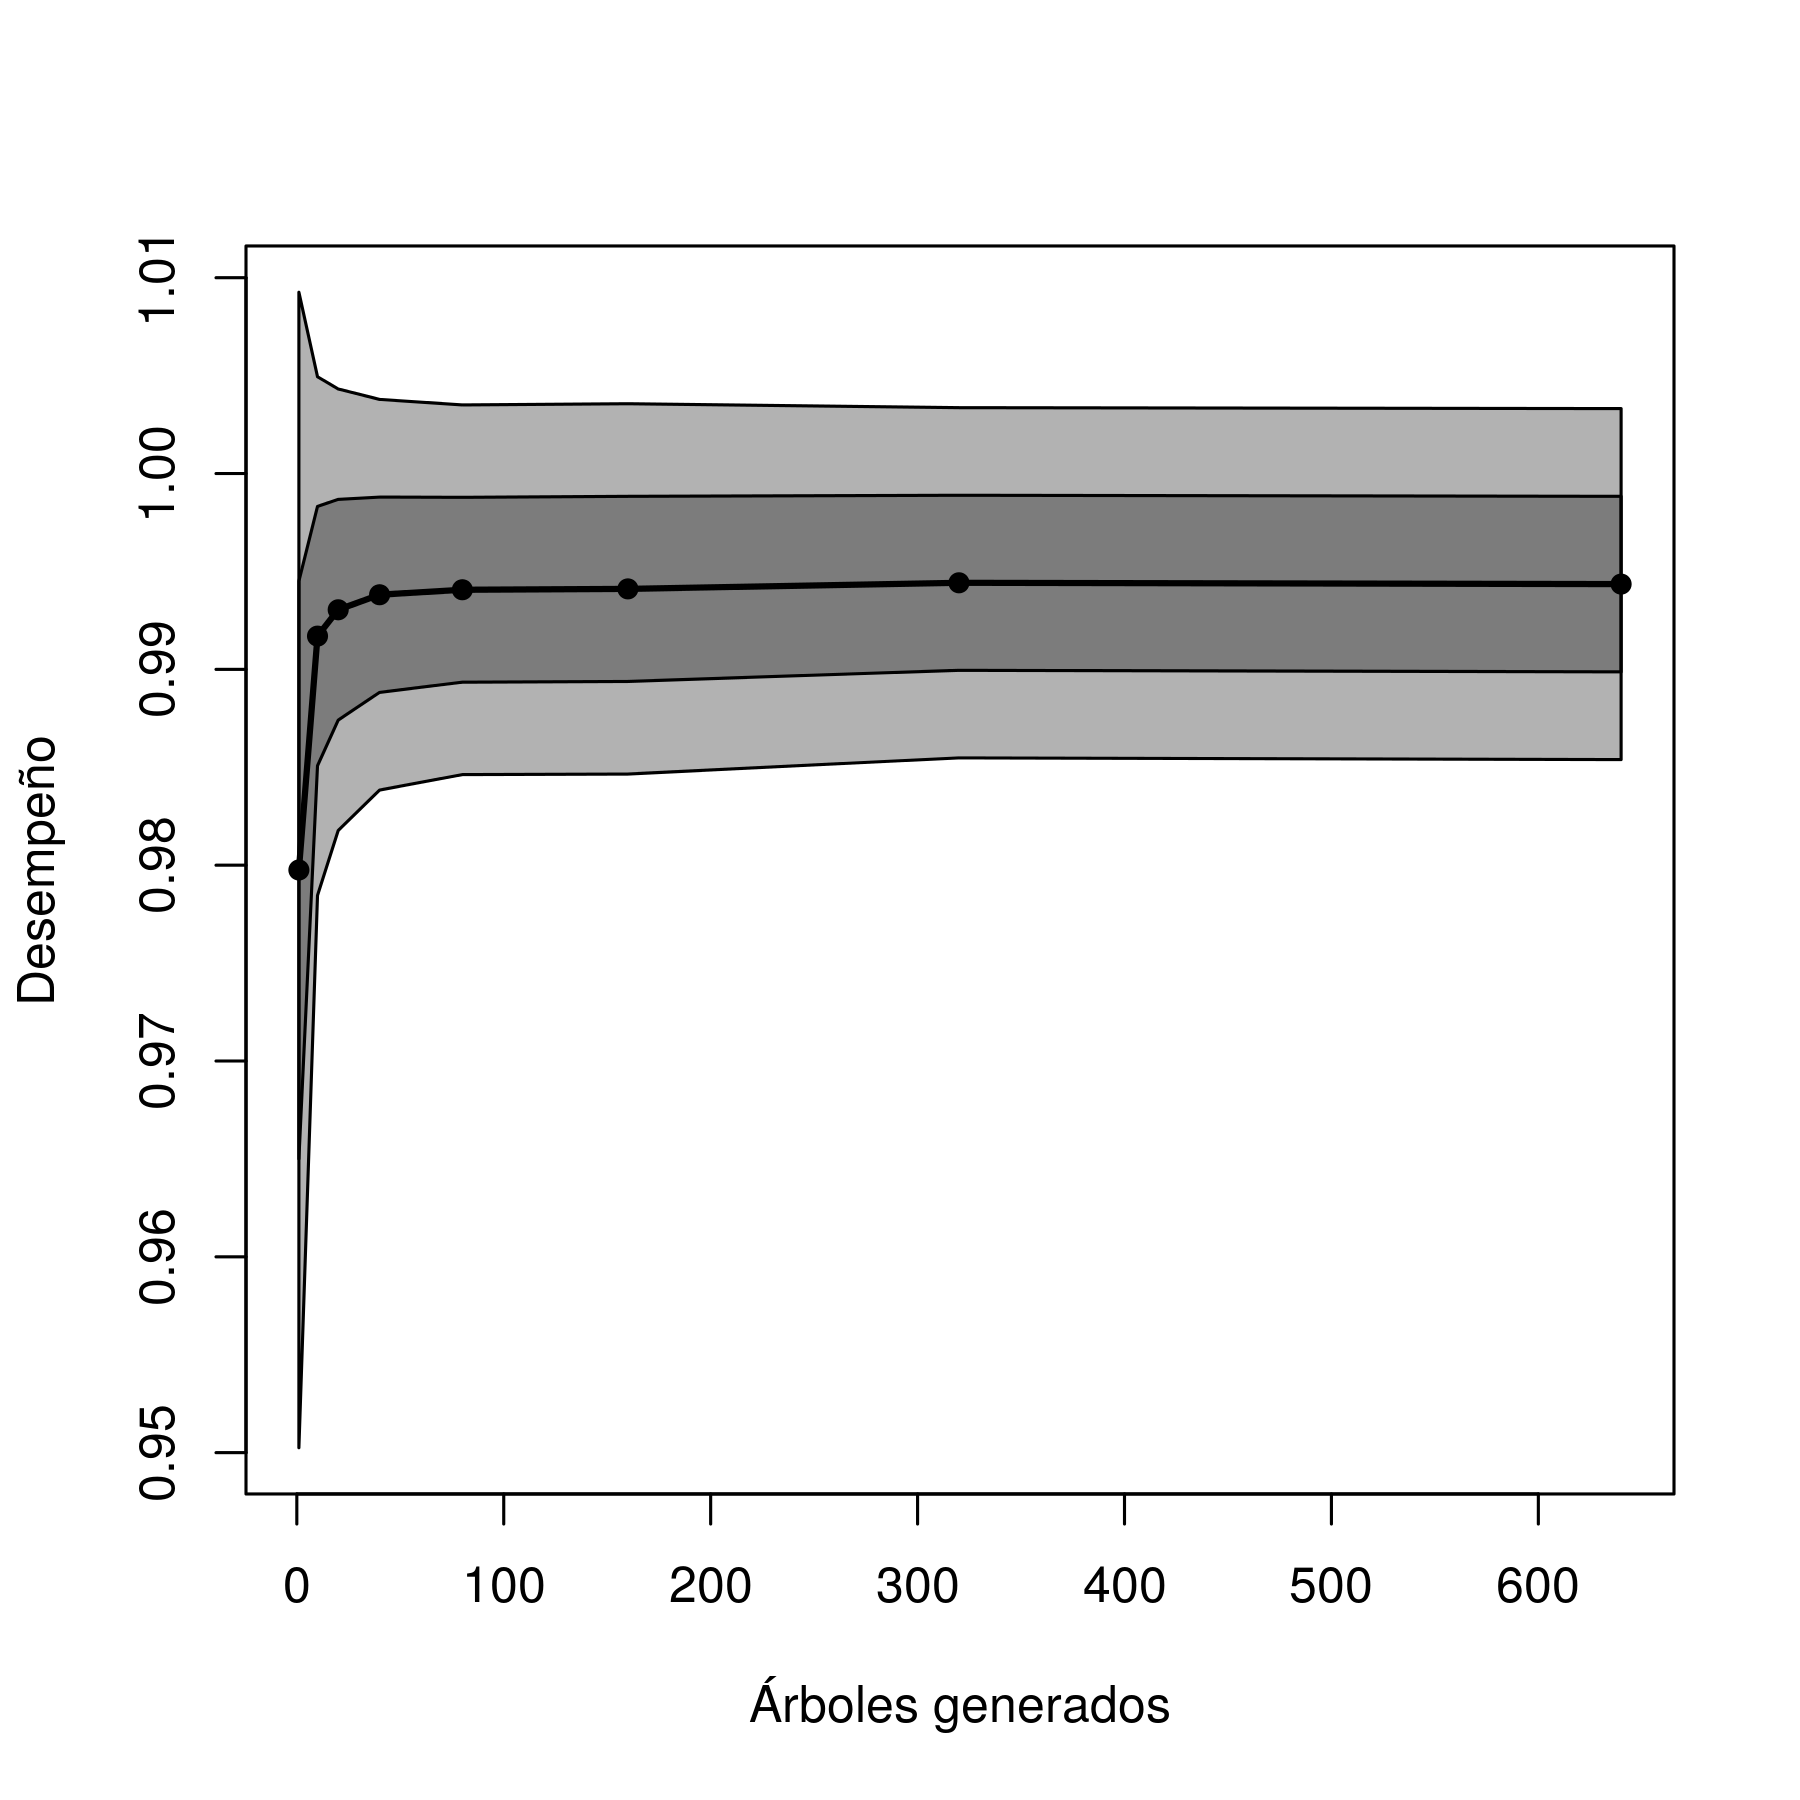
\includegraphics[width=\textwidth]{../imagenes/rf_estimators}
     \caption{}
  \end{subfigure}
  \label{fig:rf_estimators}
\end{figure}

Con 40 \'arboles probamos el desempeño 

\begin{figure}[H]
  \centering
  \begin{subfigure}[b]{0.4\textwidth}
    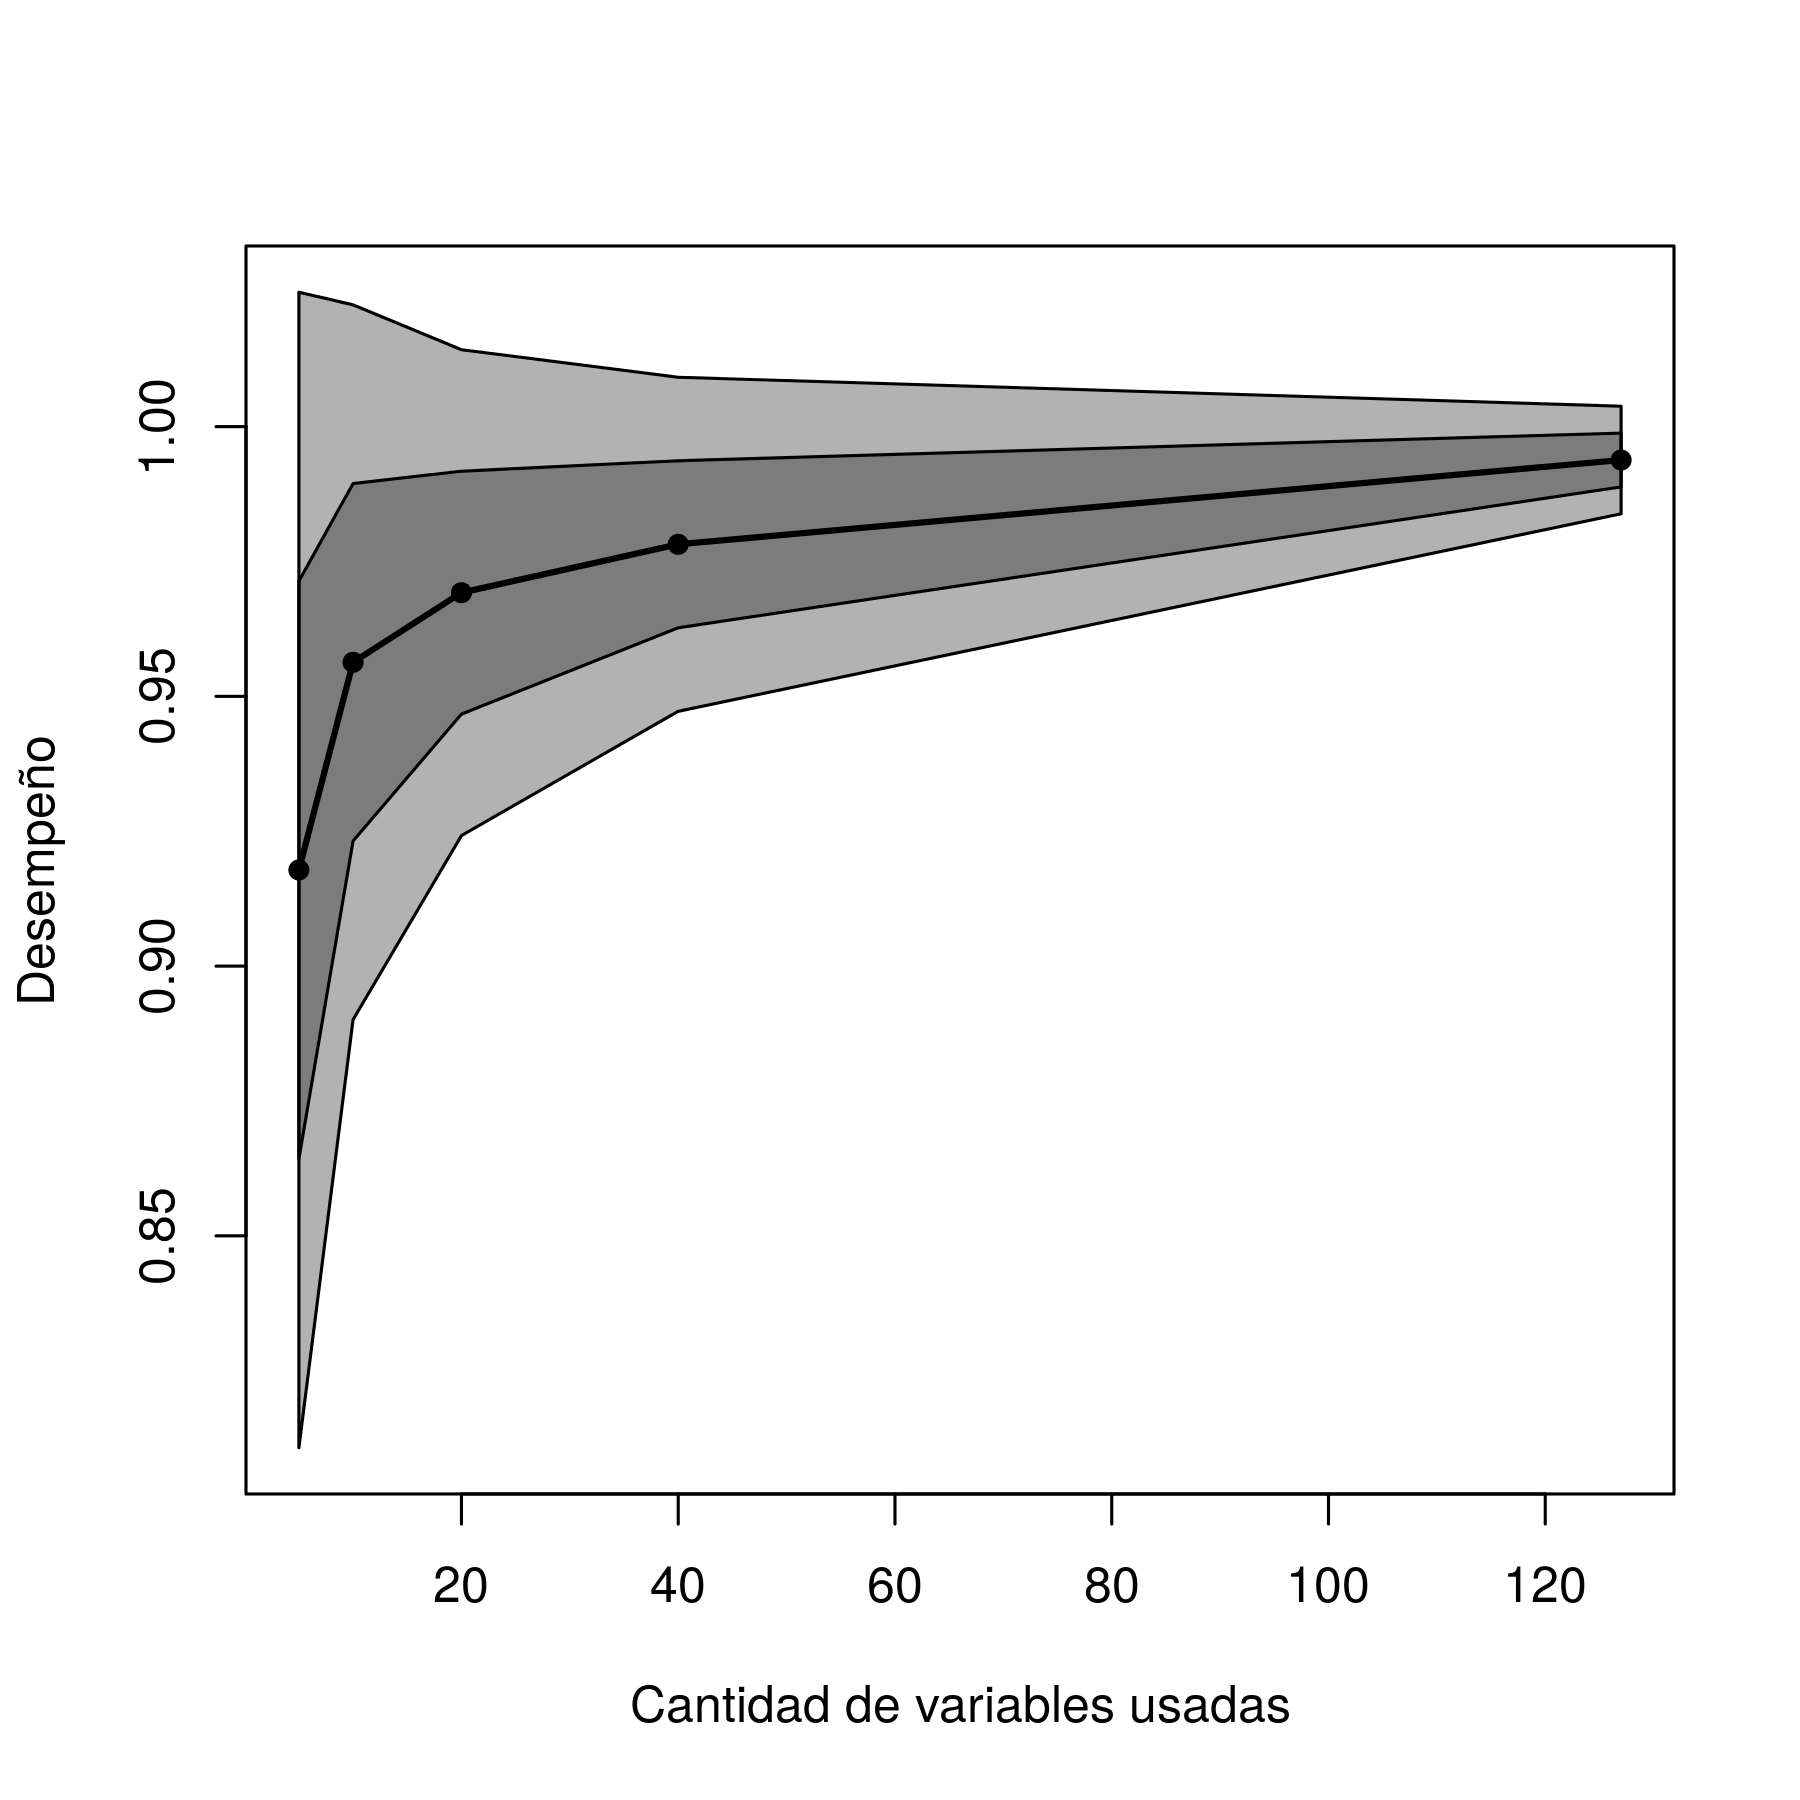
\includegraphics[width=\textwidth]{../imagenes/rf}
     \caption{}
  \end{subfigure}
  \label{fig:rf}
\end{figure}


\subsection{Suport Vector Machine. SVM.}

\par Decidimos realizar el estudio para SVM con un subconjunto del dataset original. Del tutorial de \emph{scikit-learn} (\cite{sklearn}) observamos que el tiempo de ejecución es cuadrático con el número de muestras originales, por lo cual vuelve a este método muy lento de entrenar y validar respecto de los estudiados en las secciones anteriores. Por lo tanto, con un dataset acotado a 10000 mails (50\% ham - 50\% spam) obtuvimos las eficacias de la figura \ref{fig:svm} para distintos kernels y valores del parámetro C.

\begin{figure}[H]
  \centering
  \begin{subfigure}[b]{0.4\textwidth}
    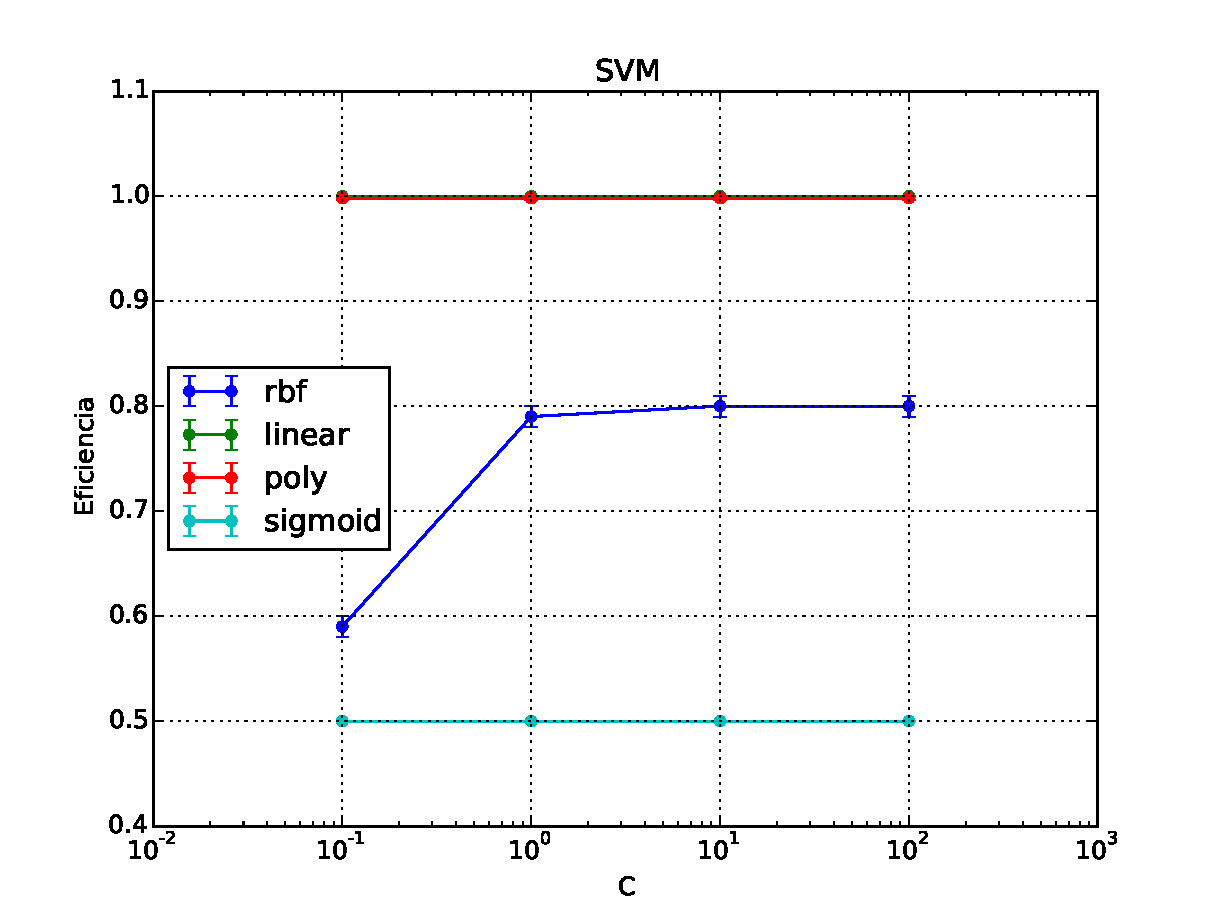
\includegraphics[width=\textwidth]{../imagenes/SVM}
     \caption{}
  \end{subfigure}
  \label{fig:svm}
\end{figure}

\par Los tiempos de ejecución para cada kernel, promediados para los valores de $C$ empleados son los siguientes:
\begin{table}[H]
\centering
\caption{}
\label{table:time_svm}
\begin{tabular}{ll}
Kernel & Tiempo (s) \\
Linear & 1850 \\
Poly (degree = 3) & 202 \\
Rbf & 192 \\
Sigmoid & 154 \\
\end{tabular}
\end{table}
De la tabla \ref{table:time_svm} y la figura \ref{fig:svm} concluímos que SVM para un los kernels \emph{linear} y \emph{poly} dan una muy buena eficacia, que el tiempo para \emph{linear} es mucho mayor que para \emph{poly}, pero que ambos casos, el tiempo de validación es claramente más alto que los otros métodos estudiados, aún al trabajar con un dataset acotado.

(SI TERMINA;, VOY A PONER SVM CON C=1 Y KERNEL = POLY CON TODA LA DATA)

\section{Reducci\'on de dimensionalidad}

\subsection{Features Ranking}

Evaluamos la ganancia de cada variable individualmente y obtuvimos el siguiente ranking. 

  \begin{figure}[H]
    \centering
    \begin{subfigure}[b]{0.4\textwidth}
      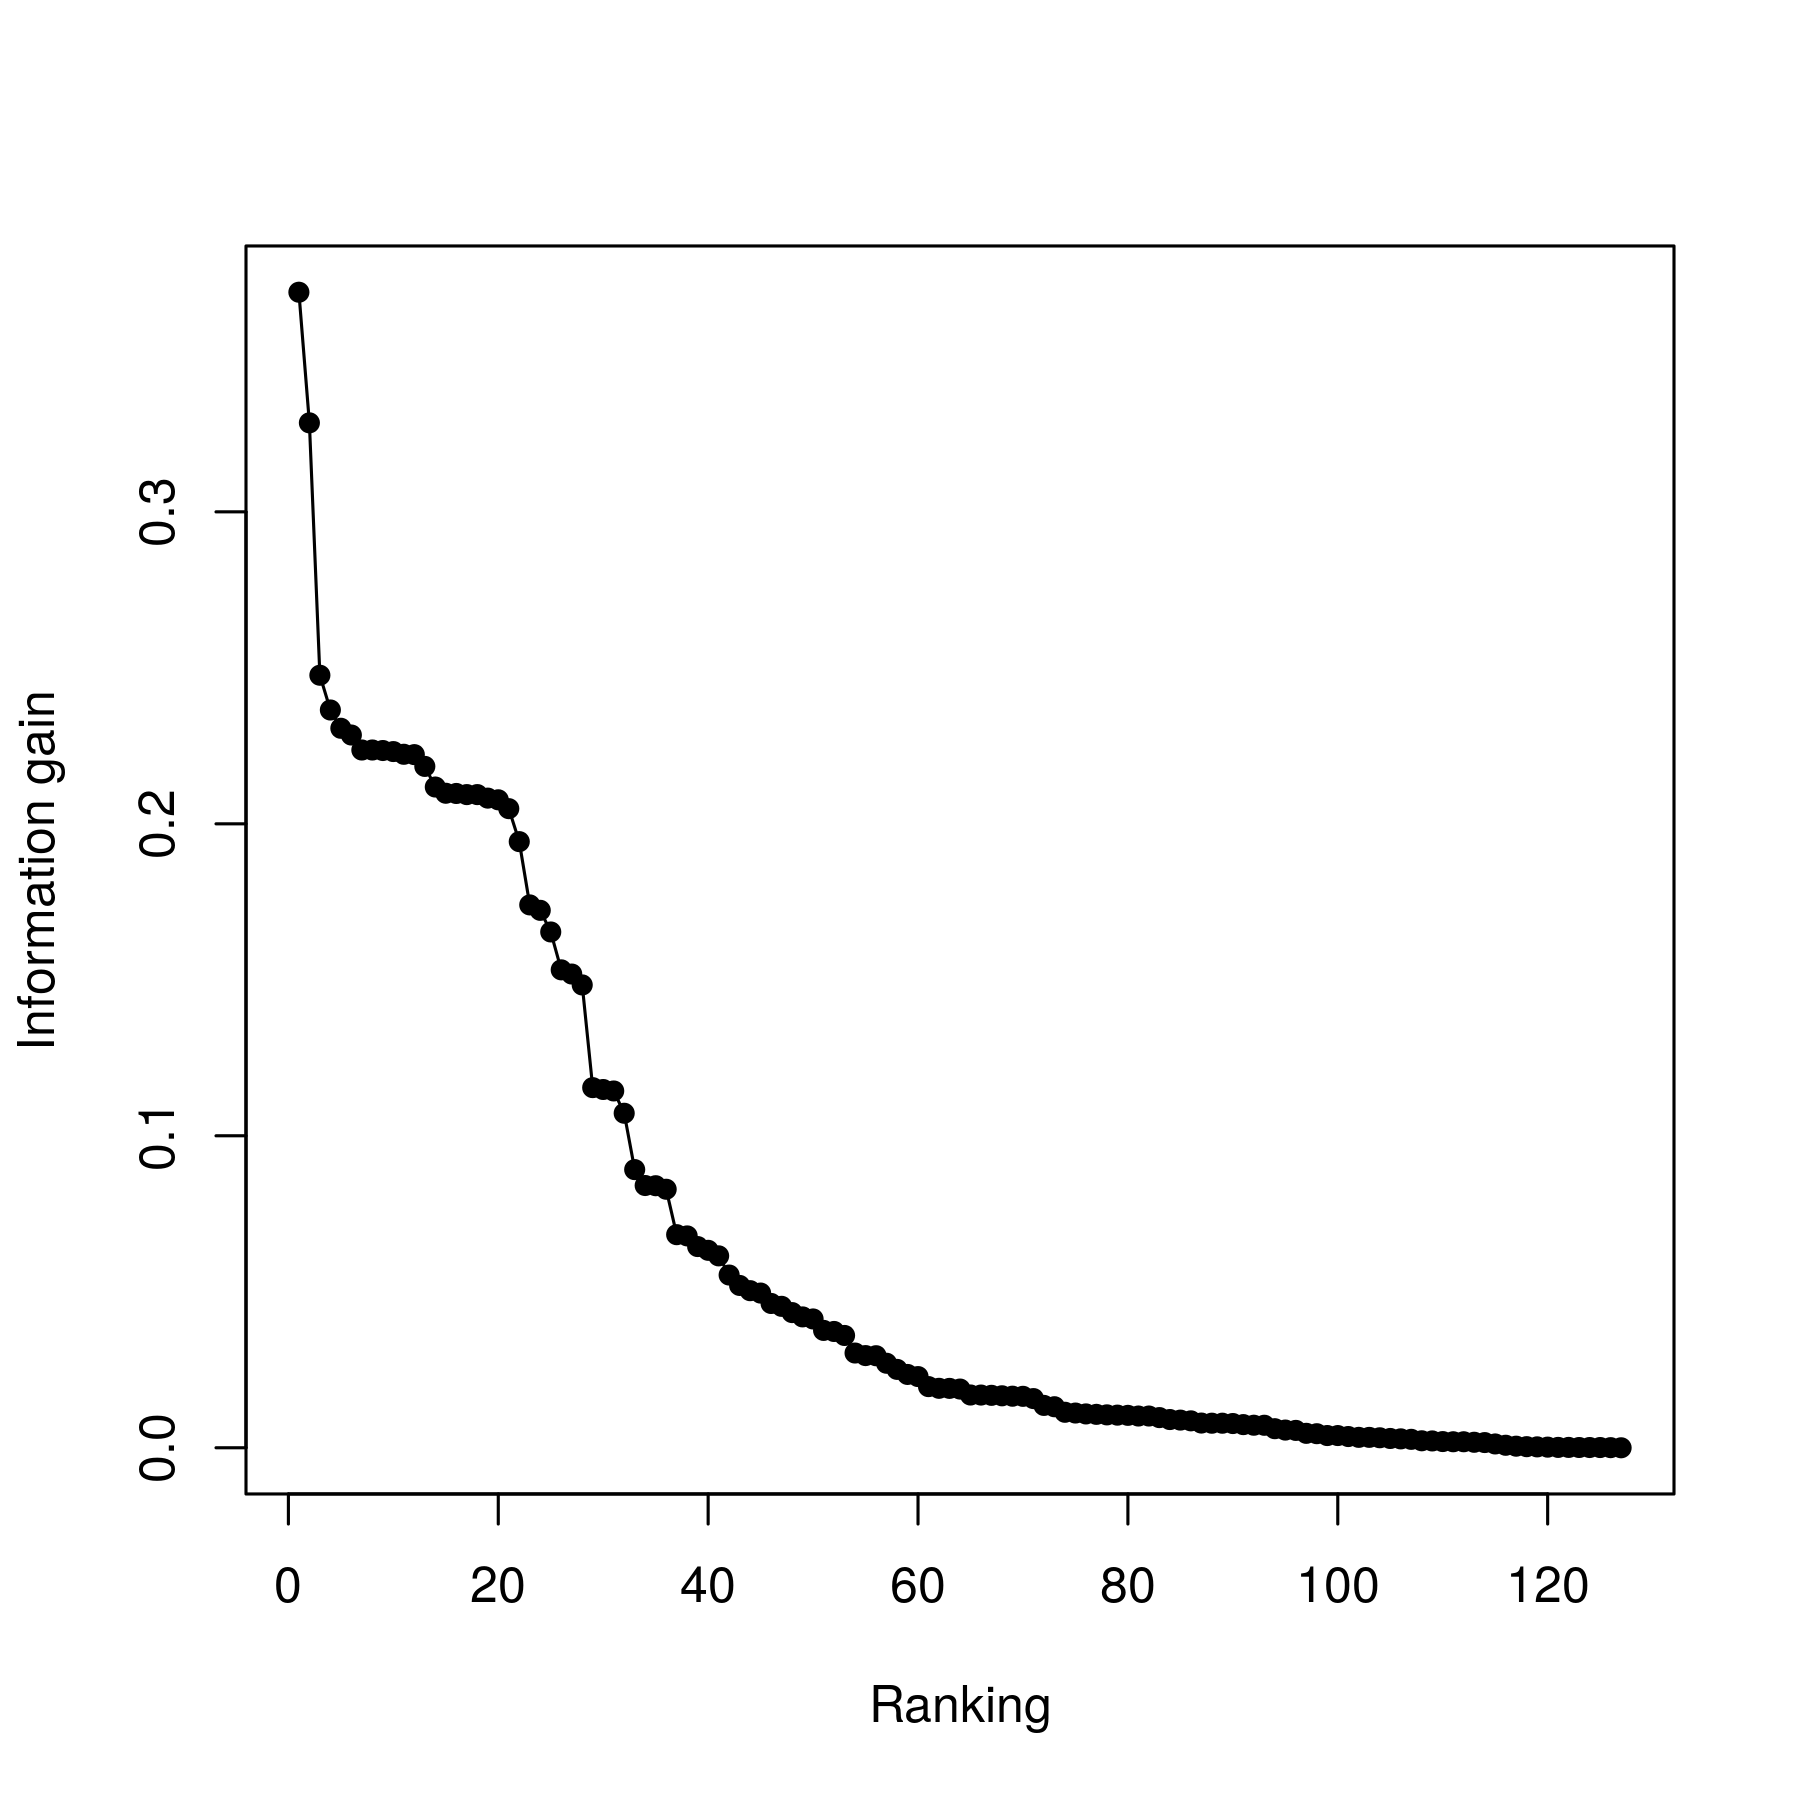
\includegraphics[width=\textwidth]{../imagenes/features_ranking}
      \caption{}
    \end{subfigure}
    \label{fig:features_ranking}
  \end{figure}

Este m\'etodo considera la dependecia de las variables. 

\subsection{Hill climbing}

Implementamos completo un algoritmo de hill climibing. Este m\'etodo de selecci\'on de variables depende de la performance resultante de aplicar a un conjunto de datos, $D$, un modelo $L$, evualuado sobre un subconjunto de atributos $S$. La vecindad de un subconjunto $s$ son todos los subconjuntos que se pueden contruir sacando de $s$ un \'unico elemento, o agregando a $s$ un \'unico elemento. Corrimos 50 procesos de hill climbing evaluando la perfomance en cada punto ejecutando un \'arbol de decisi\'on con cross validation 5-fold. Encontramos 50 \'optimos locales, sin repetici\'on. Las performance de los \'optimos locales estuvieron entre 0.88 y 0.96. Este proceso no fue suficiente para decidir por un \'unico subconjunto de atributos para la selecci\'on de atributos. 



\subsection{PCA}

\par De los atributos seleccionados, realizamos un reducción de la dimensionalidad
mediante la técnica de PCA. Dada la matriz de \emph{mails} x \emph{atributos},
calculamos la matriz de covarianza de los atributos, y realizamos una descomposición en valores singulares (SVD). La matriz de covarianza es una matriz simétrica, por lo tanto sus valores singulares coinciden con sus autovalores, que además son reales y no negativos. En la figura \ref{fig:autovalores}, observamos el valor de los mismos, ordenados de mayor a menor. 
  \begin{figure}[H]
    \centering
    \begin{subfigure}[b]{0.4\textwidth}
      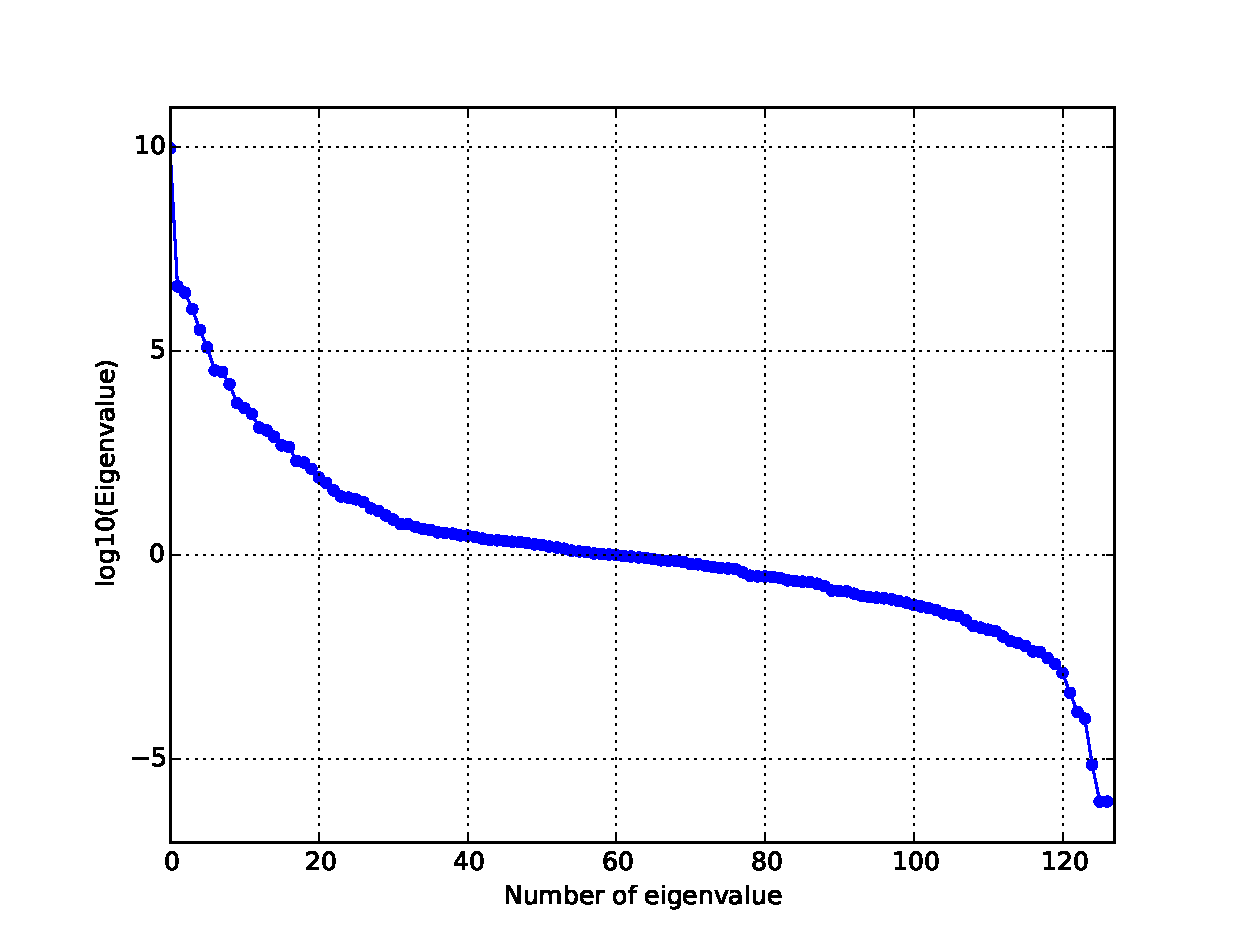
\includegraphics[width=\textwidth]{../imagenes/Autovalores}
      \caption{}
    \end{subfigure}
    \label{fig:autovalores}
  \end{figure}

\par Los autovectores obtenidos de la factorización son una combinación lineal de los atributos elegidos originalmente. Dichos autovectores pueden ser tomados como nuevos atributos, los cuales, a partir de sus autovalores asociados, sabemos en cuáles hay una mayor variabilidad de los datos. 
\par Para dar una interpretación a los nuevos atributos, observamos la representación de los autovectores en el espacio de atributos originales. Como criterio, estudiamos qué componentes tienen un valor absoluto mayor a $0.1$ en el espacio de atributos originales. En la tabla \ref{table:autovectores} mostramos el resultado para las 5 direcciones principales. De la tabla vemos que las dos direcciones principales prácticamente coindicen con dos de los atributos elegidos originalmente, asociados al formato del mail en cuestión. Los autovectores siguientes se constituyen de un grupo de términos, de los cuales el 4º y 5º autovector muestran una correlación en la terminología (o procedencia) de los miembros del grupo más visible que en el 3º autovector. 
\begin{table}
\centering
\caption{}
\label{table:autovectores}
\begin{tabular}{ll}
Autovector & Componentes principales \\
1 & Largo del documento. \\
2 & Cantidad de espacios en blanco. \\
3 & Términos: germ, hi, how, think, valuable, enron, republic, content-class, thread-index. \\
4 & Términos: x-origin, x-filename, x-cc, binary \\
5 & Términos: receive, email, upgrade, fast, spam \\
\end{tabular}
\end{table}


\section{Resultados}

\section{Discusi\'on}


\scriptsize
\bibliographystyle{splncs03}
\bibliography{aa}



\end{document}

